\documentclass[aspectratio=169]{beamer}

% parse most utf-8 correctly
\usepackage[utf8]{inputenc}

% better graphics
\usepackage{graphicx}

% beamer settings
\title{snailmail}
\author{Noah Vogt \& Simon Hammer}
\institute{Gymnasium Kirschgarten}
\usetheme{Copenhagen}

\usepackage{varwidth}

\usepackage{graphicx,calc}
\newlength\myheight
\newlength\mydepth
\settototalheight\myheight{Xygp}
\settodepth\mydepth{Xygp}
\setlength\fboxsep{0pt}

\newcommand*\inlinegraphics[1]{
    \settototalheight\myheight{Xygp}
    \settodepth\mydepth{Xygp}
    \raisebox{-\mydepth}{\includegraphics[height=\myheight]{#1}}%
}

\begin{document}
\maketitle

\begin{frame}{Inhaltsverzeichniss}
\ldots{}
\end{frame}

%\begin{frame}{Motivation}
%\begin{itemize}\pause
%    \item allgemeines Interesse\pause
%    \item fehlender Edubs-Mail-Client\pause
%    \item persönliche Bedürfnisse
%\end{itemize}

\begin{frame}{Motivation}
\begin{varwidth}{.5\textwidth}
        \begin{figure}
            \centering
            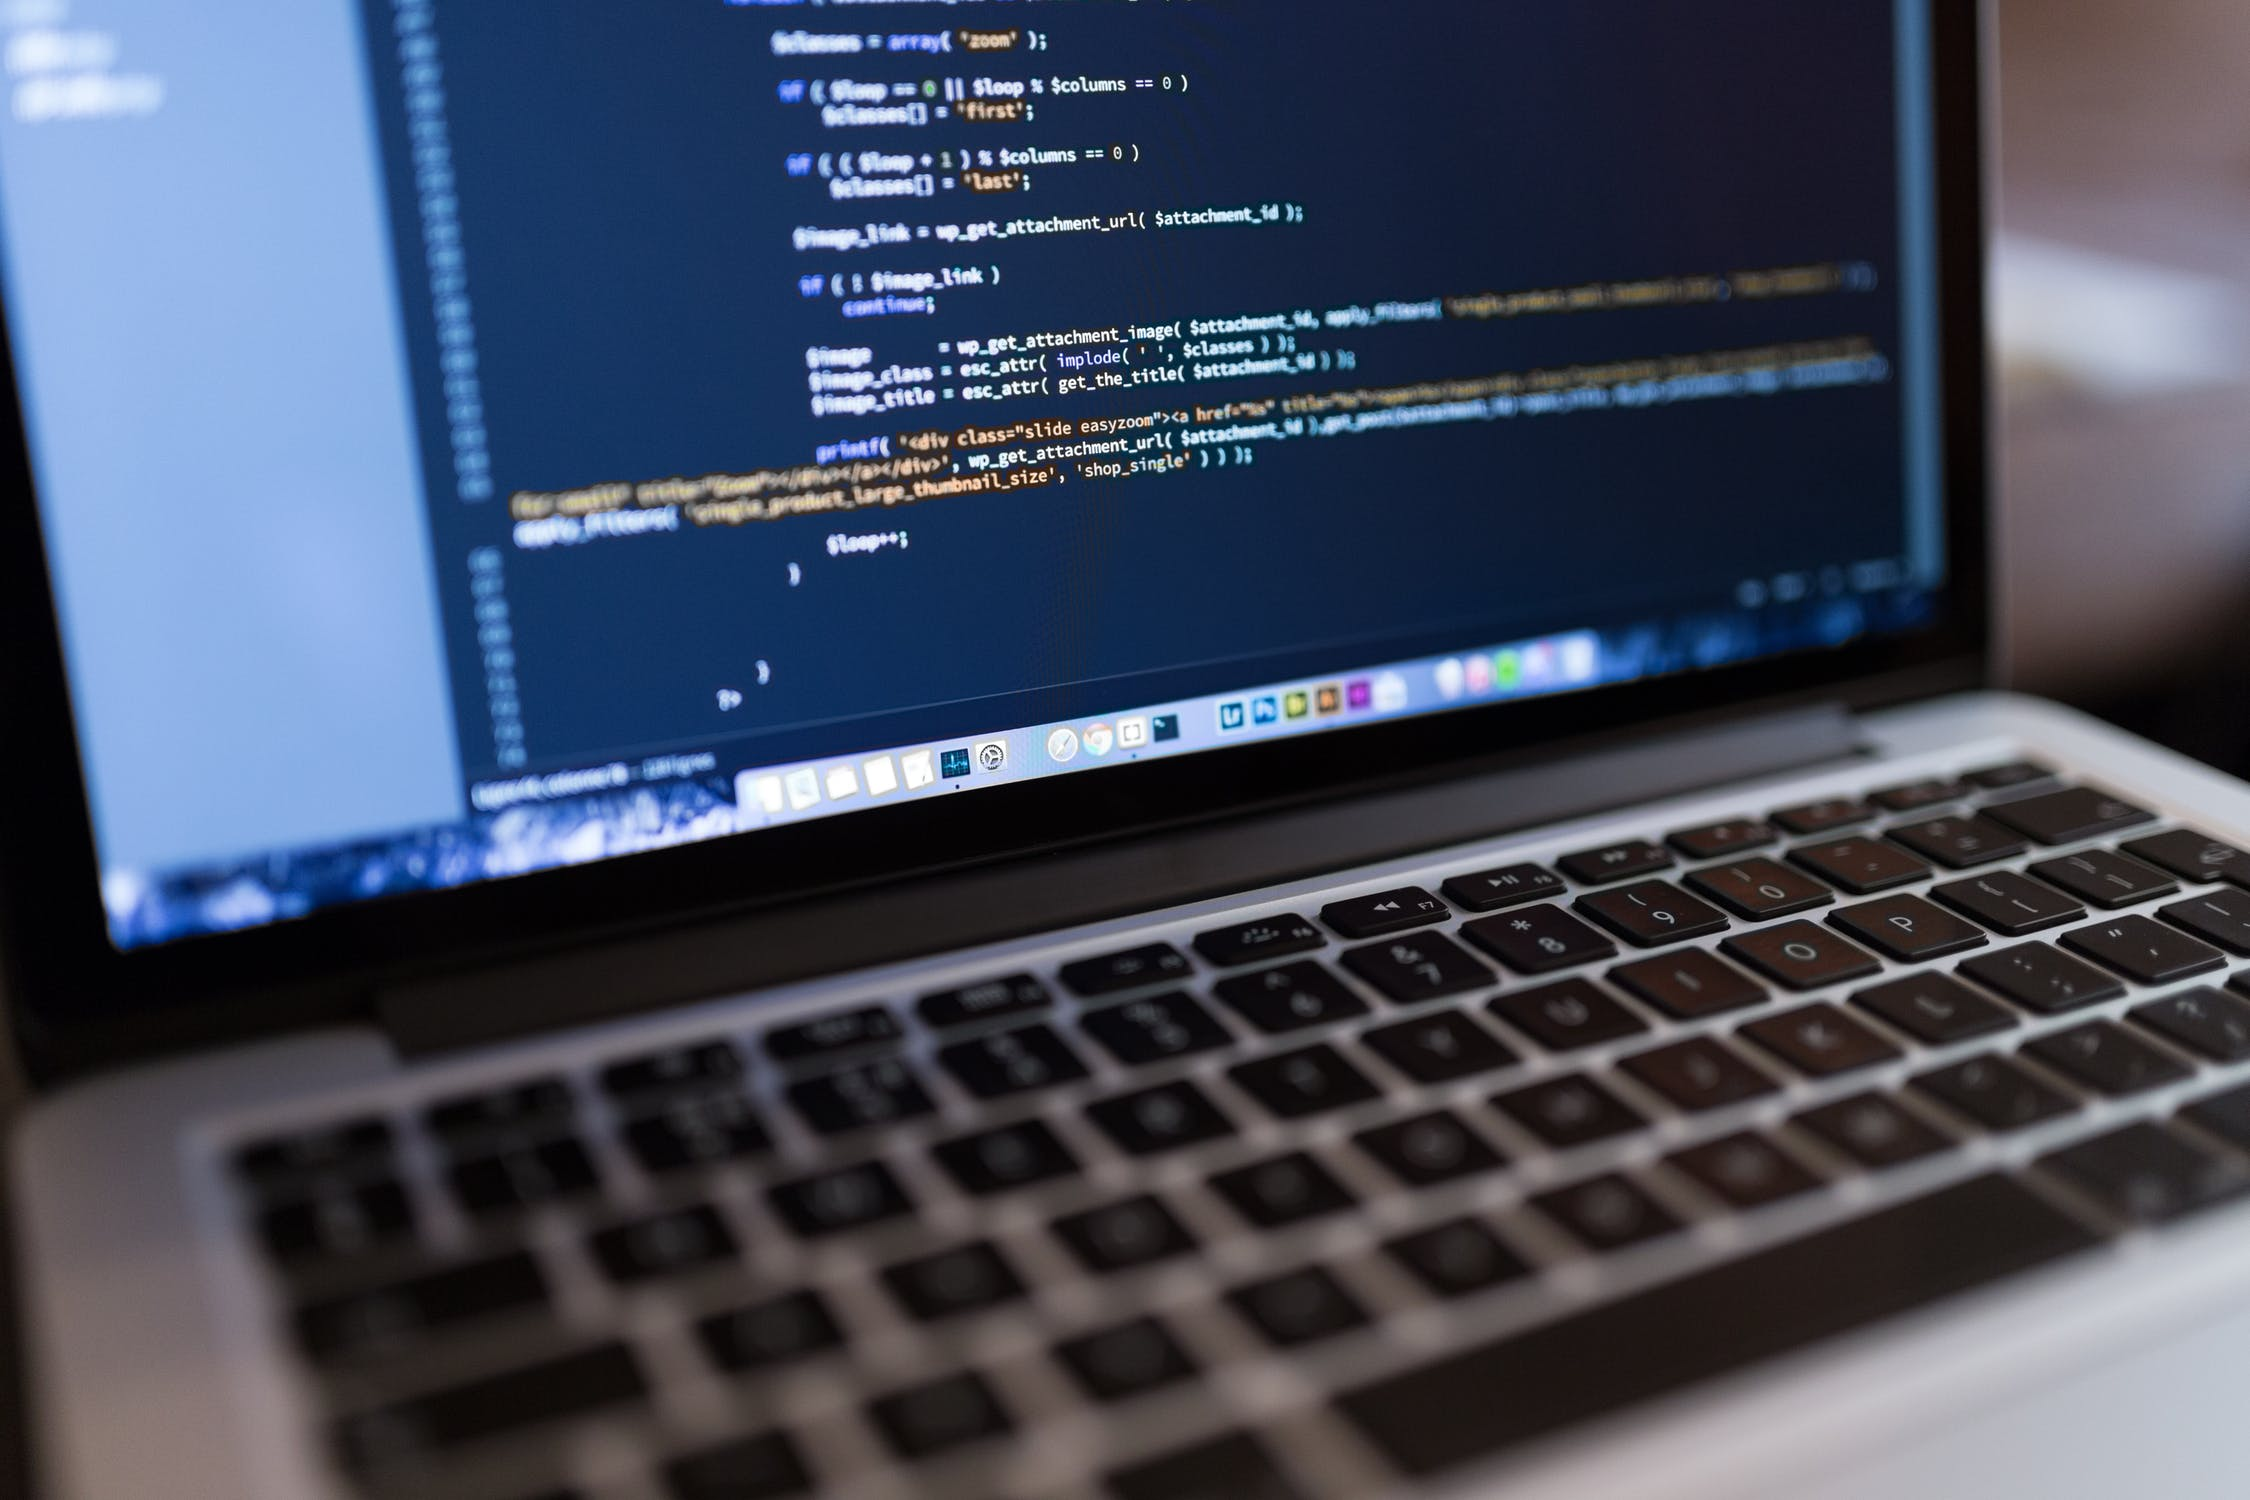
\includegraphics[width=.9\textwidth]{media/macbook.jpg}
        \end{figure}
    \end{varwidth}
    \hfill
    \begin{varwidth}{.5\textwidth}
        \begin{itemize}\pause
            \item allgemeines Interesse\pause
            \item fehlender Edubs-Mail-Client\pause
            %\item fehlender Edubs-Mail-Client\inlinegraphics{media/baslerstab-1.jpg}\pause
            \item persönliche Bedürfnisse
        \end{itemize}
    \end{varwidth} 
\end{frame}

%\begin{frame}{Ziele}
%\begin{itemize}\pause
%    \item Basisfunktionen\pause
%    \item Account Manager\pause
%    \item Design Prinzipien\pause
%    \item Schnelligkeit\pause
%    \item Mobil und Modern\pause
%    \item Einstellungen\pause
%\end{itemize}
%\end{frame}

\begin{frame}{Ziele}
\begin{varwidth}{.5\textwidth}
        \begin{figure}
            \centering
            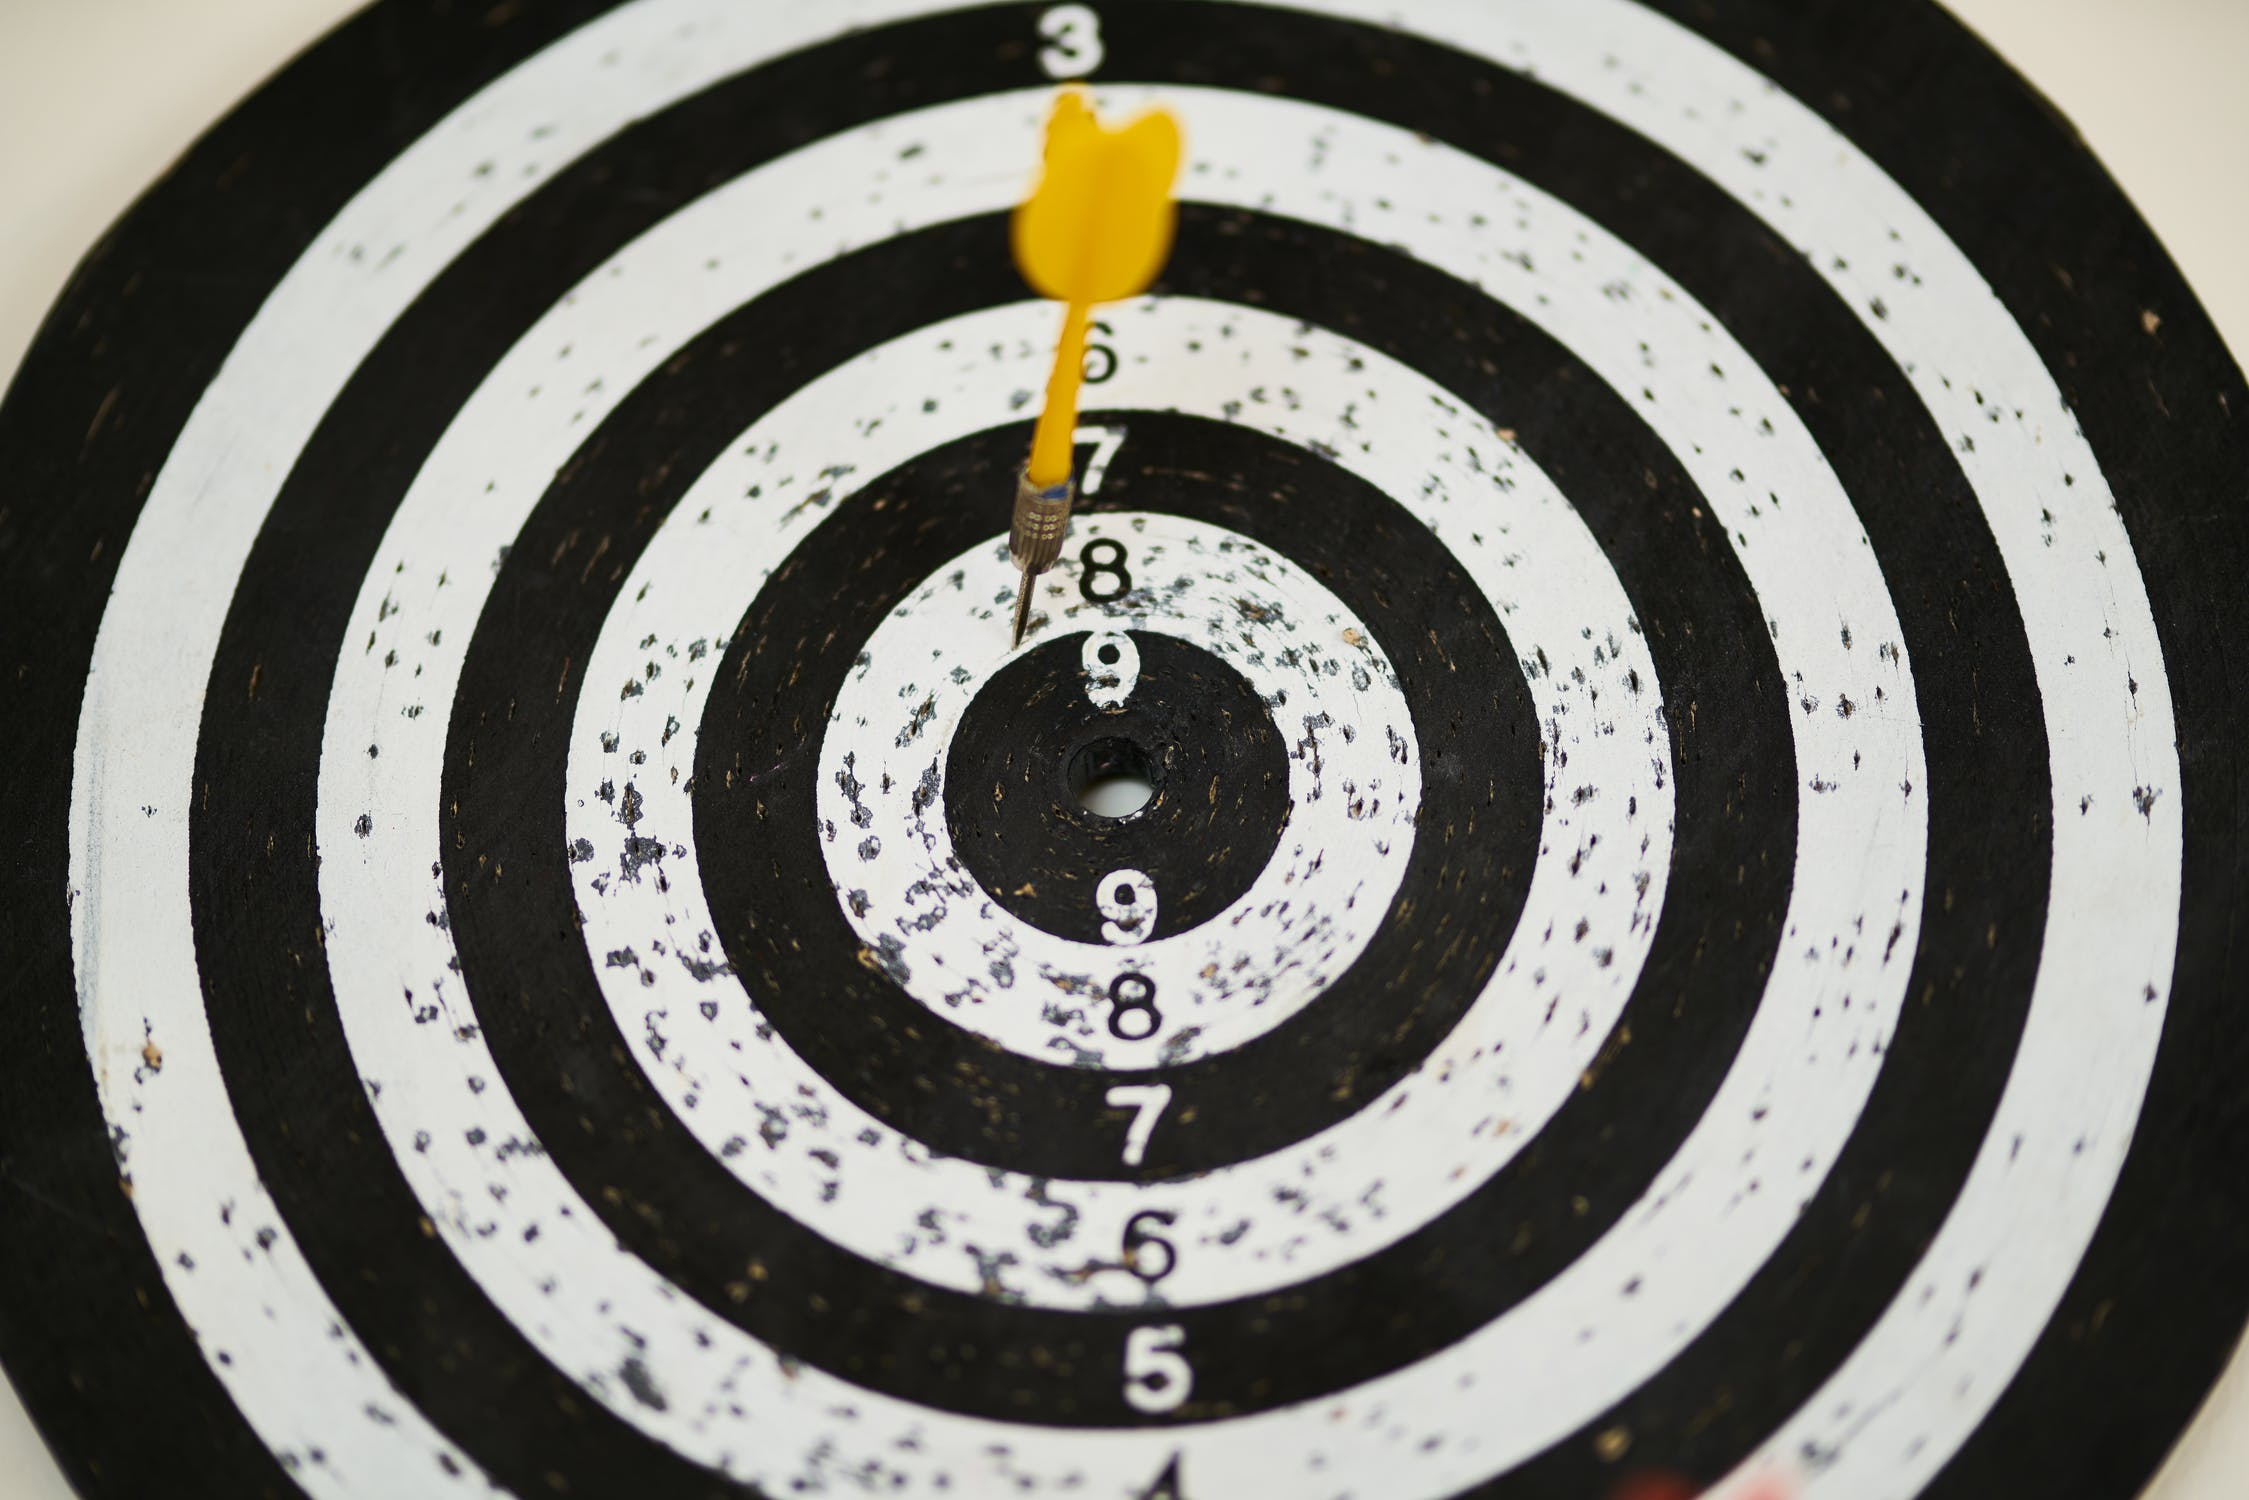
\includegraphics[width=.9\textwidth]{media/target.jpeg}
        \end{figure}
    \end{varwidth}
    \hfill
    \begin{varwidth}{.5\textwidth}
        \begin{itemize}\pause
            \item Basisfunktionen \inlinegraphics{media/mail.png} \pause
            \item Account Manager\inlinegraphics{media/business.png}\pause
            \item Design Prinzipien\inlinegraphics{media/paintbrush.png}\pause
            \item Schnelligkeit\inlinegraphics{media/run.png}\pause
            \item Mobil und Modern\inlinegraphics{media/mobile.png}\pause
            \item Einstellungen\inlinegraphics{media/settings.png}
        \end{itemize}
    \end{varwidth} 
\end{frame}

\begin{frame}{Warum Java}
\begin{varwidth}{.3\textwidth}
        \begin{figure}
            \centering
            
\includegraphics[height=.8\textheight]{media/java-logo.png}
        \end{figure}
    \end{varwidth}
    \hfill
    \begin{varwidth}{.6\textwidth}
        \begin{itemize}\pause
            \item war offizielle Sprache für Android Apps\pause
            \item abgelöst von Kotlin (seit 2019)\pause
            \item EF Informatik
        \end{itemize}
    \end{varwidth} 
\end{frame}

\begin{frame}{Demo}
\end{frame}

\begin{frame}{Was alles drin ist}
%\includegraphics<1>[height=.8\textheight]{../maturText/media/drawer.png}
%\includegraphics<2>[height=.8\textheight]{../maturText/media/inbox.jpeg}
%\includegraphics<3>[height=.8\textheight]{../maturText/media/emailWriter.png}
\end{frame}

\begin{frame}{allg Struktur}
\centering
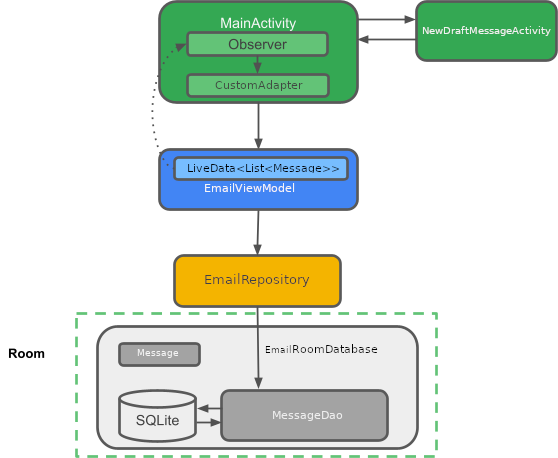
\includegraphics[height=.7\textheight]{../maturText/media/AppStructure.png}
\end{frame}

\begin{frame}{Database}
\begin{block}{allgemein}
\end{block}

\begin{block}{in der app}
\end{block}
\end{frame}

\end{document}
